\chapter{Experiments \& Results}\label{ch:Experiments & Results}

In this pivotal chapter, we embark on a journey through the experiments and results that form the core of this thesis. Our exploration begins with the initial steps of setting up the dataset using the NeRF original codebase, and it culminates in the realization of our ultimate thesis goal. Within these pages, we delve into the intricacies of each experiment, documenting both the successes and setbacks encountered along the way.

\section{Preliminary Evaluation of NeRFStudio}


Our initial foray into Neural Radiance Fields (NeRF) began with the exploration of NeRFStudio, a crucial platform for understanding and utilizing NeRF techniques. This exploration included setting up NeRFStudio and employing their publicly available datasets. The outcomes of these initial trials closely matched the results documented in the original NeRF paper, confirming the tool's effectiveness and reliability. This preliminary phase was instrumental in establishing a solid foundation for our subsequent, more in-depth experiments involving custom datasets. These early trials with NeRFStudio were pivotal in shaping our approach and understanding of NeRF's capabilities and limitations.

\subsection{Utilization of Custom Datasets in NeRFStudio}


In our quest to deepen our understanding of Neural Radiance Fields, we initiated an experiment using a custom dataset. This dataset comprised a small collection of images, numbering around 5 to 6, all depicting the same object - a clock. These images were captured from various angles using an iPhone X, resulting in high-quality images with clear details. Each image was sizeable, ranging from 9MB to 11MB, and shared the same resolution of 3024 X 4032 pixels. This collection of images, distinct in their clarity and focus on the singular object, provided a valuable resource for our study. 
\vspace{10pt}

The experiment with the dataset in \ref{fig:Clock Dataset} revealed limitations in the NeRF and NeRFStudio models. It became evident that using a small dataset of only 5 to 6 images led to suboptimal reconstruction quality. The images, despite their clarity, resulted in a blurry reconstruction when processed through these models. This outcome highlighted the significant impact of dataset size on the effectiveness of NeRF-based reconstructions, emphasizing the need for larger datasets to achieve higher quality in 3D model reconstruction.

\begin{figure}[H]
    \centering
    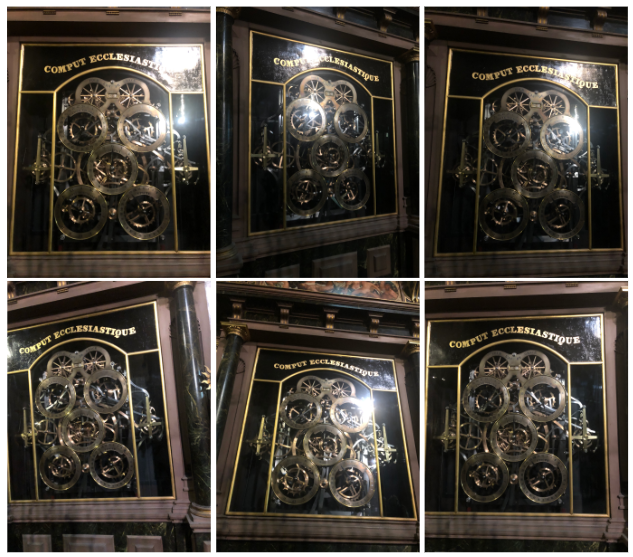
\includegraphics[width=0.6\textwidth]{img/Clock dataset.png}
    \caption{Sample Image from the Clock Dataset.}\label{fig:Clock Dataset}
\end{figure}




\subsection{Scaling Dataset Size}


In our subsequent experiment, we employed a larger custom dataset as detailed in \ref{fig:Dataset of 2D Images from Various Camera Positions}. This dataset was comprised of over 50 high-resolution images of a single object, captured using an iPhone X, with each image size ranging between 10 to 15 MB. The high-quality nature of these images was evident, as even when magnified three times, the images remained clear, with no blurriness. This experiment emphasized the importance of dataset quality and size in achieving optimal reconstructions with NeRF models.

\begin{figure}[thbp]
    \centering
    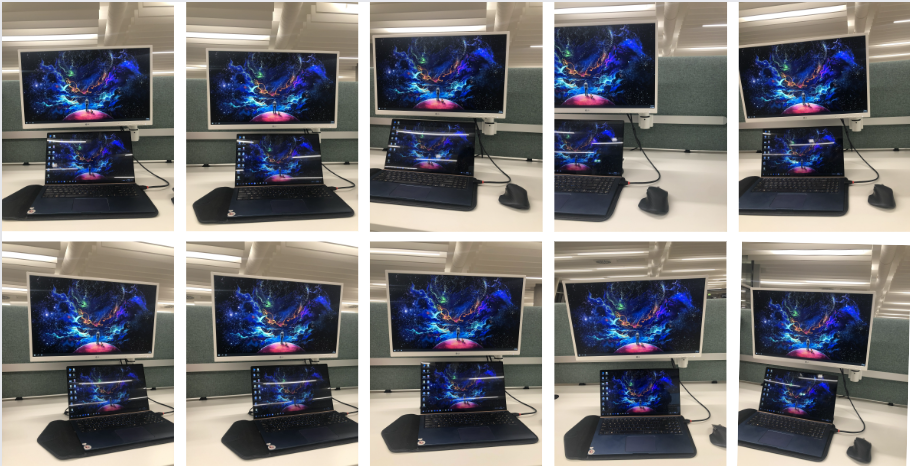
\includegraphics[width=0.8\textwidth]{img/Nerf data.png}
    \caption{Dataset of 2D Images from Various Camera Positions.}\label{fig:Dataset of 2D Images from Various Camera Positions}
\end{figure}

The results of this experiment demonstrated a significant improvement in reconstruction quality compared to the smaller dataset. 

\begin{figure}[thbp]
    \centering
    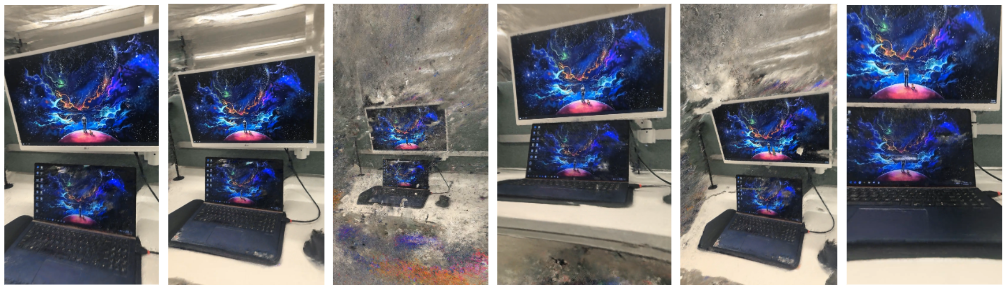
\includegraphics[width=0.8\textwidth]{img/Nerf Result.png}
    \caption{Still Frames from Video Generated by NeRFStudio Using 2D Images.}\label{fig:Still Frames from Video Generated Using 2D Images with New Camera Angle}
\end{figure}
\vspace{10pt}
The still frames from the generated video provided insight into the potential of NeRF when working with datasets that meet the minimum image count requirements. Through these experiments, we gained valuable insights into the capabilities and limitations of Neural Radiance Fields, emphasizing the significance of dataset size. These initial steps set the stage for further exploration and optimization in subsequent experiments.


\section{Exploration of TEM Image Experiments}
In this experiment, we ventured into the realm of Transmission Electron Microscopy (TEM) images, a domain known for its unique challenges in image reconstruction. Armed with a better understanding of NeRFStudio, we set out to apply Neural Radiance Fields (NeRF) to our original TEM dataset.
\vspace{10pt}

Our initial attempt involved training NeRFStudio with Dataset 1, comprising TEM images of our target subject. However, our efforts encountered an unexpected obstacle. Within a matter of minutes, an error emerged, indicating that COLMAP was unable to create the "transforms.json" file, rendering it impossible to proceed with training.

\begin{figure}[H]
    \centering
    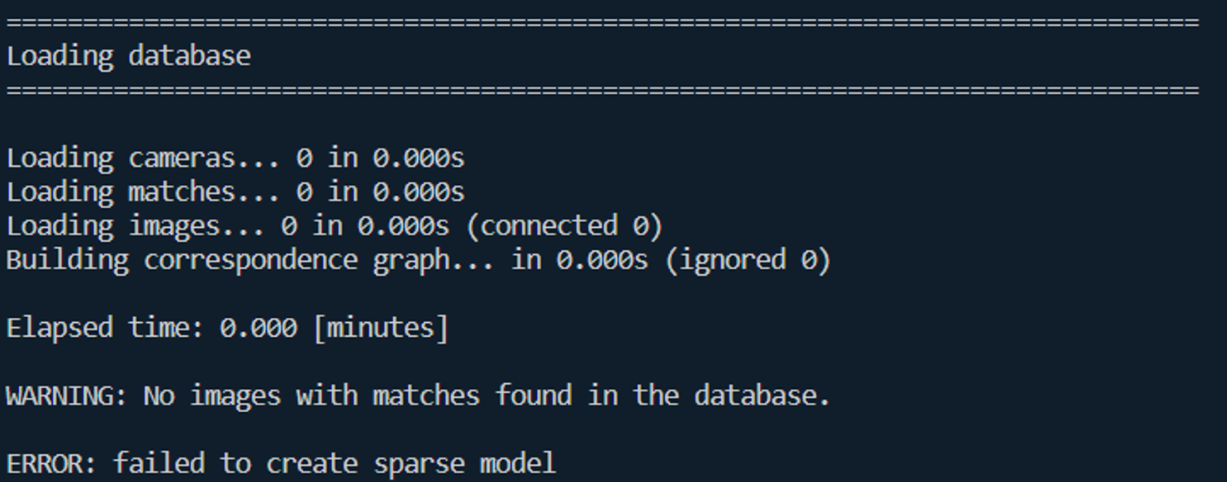
\includegraphics[width=1\textwidth]{img/Colmap error.png}
    \caption{COLMAP Error During Training.}\label{fig:Colmap error}
\end{figure}

The underlying challenge became apparent—TEM images, characterized by their inherent noise and low quality, posed a formidable hurdle. In the context of NeRF, precise camera position information is essential for successful 3D image generation from 2D inputs. Unfortunately, the noise and quality limitations of TEM images made it extremely challenging for NeRFStudio, utilizing the Nerfacto model, to reconstruct accurate camera positions, resulting in the encountered issues.


\section{Exploring Alternative Nerf Models for TEM Images}
Recognizing the limitations of NeRFStudio with TEM images, we embarked on a quest to discover alternative Nerf models that might better address the challenges posed by TEM data. Our journey into the realm of Neural Radiance Fields led us to experiment with various models, each with its unique characteristics and capabilities. In the following table, we summarize the Nerf models we explored and the specific limitations we encountered when working with TEM images:

\begin{table}[H]
    \centering
    \begin{tabular}{|c|c|}
        \hline
        \textbf{Nerf Models} & \textbf{COLMAP Limitation with TEM Images} \\
        \hline
        NeRFStudio(Nerfacto) & Dependency on COLMAP \textcolor{red}{\ding{55}} \\
        \hline
        LeRF & Dependency on COLMAP  \textcolor{red}{\ding{55}}\\
        \hline
        Mip-NeRF & Dependency on COLMAP  \textcolor{red}{\ding{55}}\\
        \hline
        Instant-NGP & Dependency on COLMAP  \textcolor{red}{\ding{55}}\\
        \hline
        MultiNeRF & Dependency on COLMAP \textcolor{red}{\ding{55}} \\
        \hline
        NanNeRF & Dependency on COLMAP \textcolor{red}{\ding{55}} \\
        \hline
        NeRF in the Dark & Dependency on COLMAP  \textcolor{red}{\ding{55}}\\
        \hline
        IBRNeRF & Dependency on COLMAP   \textcolor{red}{\ding{55}}\\
        \hline
        RefNeRF & Dependency on COLMAP \textcolor{red}{\ding{55}}\\
        \hline
        SCNeRF & Dependency on  COLMAP \textcolor{red}{\ding{55}}\\
        \hline
        gNeRF & Dependency on  COLMAP \textcolor{red}{\ding{55}}\\
        \hline
        NeRFMM & Not Dependent on  COLMAP \textcolor{green}{\ding{51}}\\
        \hline
    \end{tabular}
    \caption{Summary of Nerf Models Experimented with TEM Images.}
    \label{tab:NerfModelsTEM}
\end{table}


This research, we delved into various Nerf models to address the specific challenges presented by TEM data, particularly focusing on achieving accurate 3D reconstructions. Most existing models were constrained by their reliance on COLMAP, a limitation that often hindered their effectiveness with TEM data. Our exploration led us to NeRFMM, a notable model that operates independently of COLMAP, offering a significant breakthrough for TEM image reconstruction. Encouraged by the success of NeRFMM, we extended our search to include the latest advancements in Nerf technology, seeking models with similar capabilities and compatibility with TEM data. Among these, LUNeRF emerged as a particularly promising model, demonstrating potential in preliminary assessments. However, the lack of public access to LUNeRF's codebase has been a barrier, limiting our ability to fully explore and validate its applicability in the context of TEM data analysis. This ongoing exploration underlines the dynamic nature of our research and the continual search for innovative solutions in the field of 3D image reconstruction.

\clearpage
\section{Exploration of COLMAP Alternatives for TEM Images}
Recognizing that nearly 95\% of our attempts to apply NERF models to TEM images resulted in failure, we conducted an in-depth investigation into the underlying issue. It became apparent that COLMAP played a pivotal role as a critical dependency in these failures. Our primary goal was to identify alternative software tools capable of processing TEM images and generating the camera's exact positions or an equivalent format, which could subsequently be converted into a transform.json file. Such a file format held the potential to enable the execution of NERF models that were originally designed for COLMAP compatibility.

\vspace{10pt}
Our experiment involved rigorously testing four different software alternatives—IMOD, SerialEM, TomoPy, and Scipion—each with its unique capabilities in image processing. The critical criteria for these tests were the software's ability to handle the specific data format of TEM images and their compatibility with the transform.json file format, a necessity for NERF models.
    
    \begin{table}[H]
        \centering
        \begin{tabular}{|c|c|}
            \hline
            \textbf{COLMAP Alternatives} & \textbf{Result with our TEM Images} \\
            \hline
            IMOD & Didn't work \textcolor{red}{\ding{55}} \\
            \hline
            SerialEM & Didn't work \textcolor{red}{\ding{55}} \\
            \hline
            TomoPy & Didn't work \textcolor{red}{\ding{55}} \\
            \hline
            Scipion & Didn't work \textcolor{red}{\ding{55}} \\
            \hline
        \end{tabular}
        \caption{Summary of COLMAP Alternatives Experimented with TEM Images.}
        \label{tab:COLMAPAlternativesTEM}
    \end{table}
    

Our exploration into COLMAP alternatives for TEM data aimed to find tools for successful 3D reconstructions. We tested IMOD, SerialEM, TomoPy, and Scipion, each known for specific imaging strengths, to see if they could replace COLMAP. However, these alternatives fell short, struggling with TEM image specifics required for NERF modeling, such as precise camera positioning and compatibility with transform.json file format.

\vspace{10pt}
This led to the realization that the uniqueness of TEM images demands a novel approach, not just a replacement for COLMAP. We then shifted our focus to NeRFMM, a promising framework better suited for TEM images. Although not completely independent of COLMAP, NeRFMM represented a significant step forward, offering a new pathway for our research in applying NERF models to TEM data.  

\clearpage

\section{Experimental Analysis with TEM Dataset 3}
In our study, we worked with eight distinct datasets, each offering different complexities. This section outlines the development of our entire architecture, as illustrated in Figure \ref{fig:ThesisArchitecture}, from inception to completion. To streamline the experimental process, we chose \textbf{Dataset 3} (see Figure \ref{fig:TEM Dataset 3}) as the primary focus for in-depth analysis. Our methodology involved initially tailoring the model and its hyperparameters to \textbf{Dataset 3}, ensuring optimal performance. Once satisfactory results were obtained with this dataset, we then extended the same model configuration to the other datasets. This strategy allowed for a thorough and consistent evaluation of the model's effectiveness across various datasets.

\vspace{10pt}

In this phase of our research, we present the cumulative results of our experiments, from model development to post-processing with denoisers and ESRGAN. We successfully improved the image quality across all datasets, achieving impressive metrics such as a PSNR value exceeding 38.70 and an SSIM value of approximately 0.95. These improvements marked a significant enhancement compared to the initial metrics, which started at 28 PSNR and 0.46 SSIM for Dataset 2.


\subsection{Dataset 3: Training with 200 Epochs}

\begin{figure}[H]
    \centering
    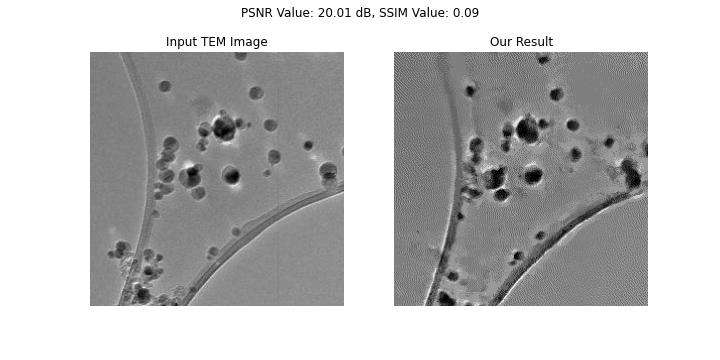
\includegraphics[width=0.8\textwidth]{img/Dataset_3_with_200_epochs.jpg}
    \caption{Dataset 3 with 200 epochs.}\label{fig:Dataset_3_with_200_epochs.jpg}
\end{figure}

These results represent the preliminary stage of our model's development, indicating a PSNR value of 20.01 and an SSIM value of 0.09. During this initial phase, our model demonstrated the capability to enhance image edges and reduce noise compared to the ground truth image.

\subsection{Dataset 3: Training with 10,000 Epochs}

\begin{figure}[H]
    \centering
    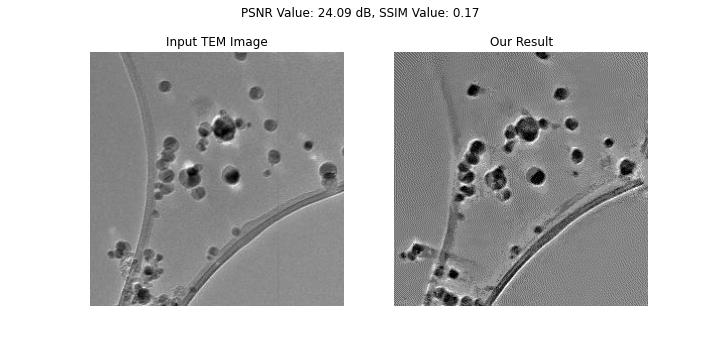
\includegraphics[width=1\textwidth]{img/Dataset_3_with_10000_epochs.jpg}
    \caption{Dataset 3 with 10,000 epochs.}\label{fig:Dataset_3_with_10000_epochs.jpg}
\end{figure}
\begin{figure}[H]
    \centering
    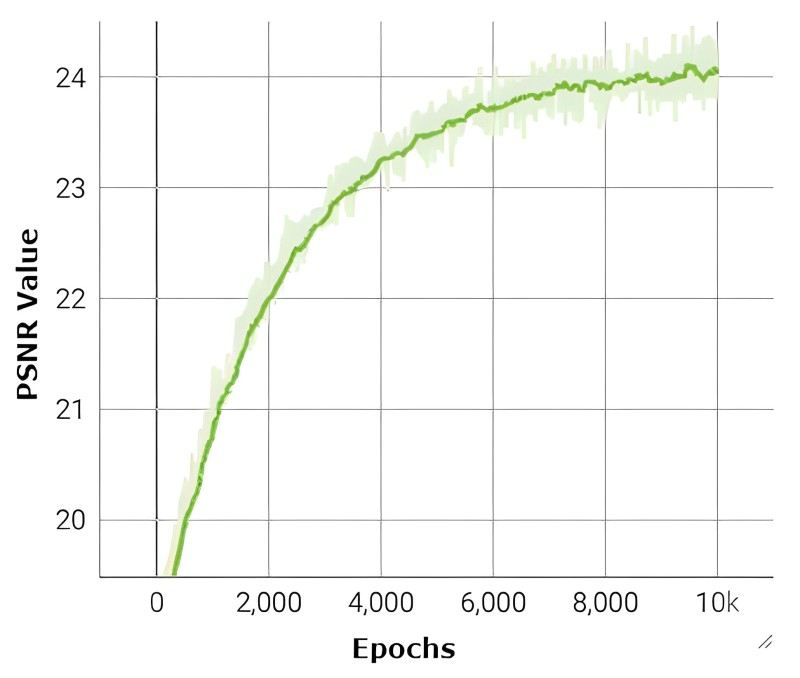
\includegraphics[width=.6\textwidth]{img/10K Psnr graph.jpg}
    \caption{Progression of PSNR values over 10,000 epochs for Dataset 3}\label{fig:Dataset 3 0 to 10000 epochs PSNR values}
\end{figure}

After undergoing an extensive training process spanning 10,000 epochs over a duration of roughly 8 to 9 hours, the model demonstrated a substantial enhancement in its performance. This intensive training phase led to a notable increase in the PSNR value, escalating from 20.01dB to 24.09dB, as depicted in \ref{fig:Dataset 3 0 to 10000 epochs PSNR values}, which denotes a significant improvement in image quality. While the PSNR value showed considerable improvement, the SSIM value, indicative of image structural similarity, remained relatively stable, exhibiting significant variations. This pattern suggests that despite the improved PSNR, the model consistently maintained the structural integrity of the images throughout the training period.


\subsection{Dataset 3: Camera Pose Optimization after 10,000 Epochs}


Figure \ref{fig:Camera Position Optimization} showcases the model's gradual improvement in optimizing camera positions across 10,000 training epochs. Starting from an initial position near (0,0) at epoch 0, the model progressively refines its camera parameter adjustments. This steady enhancement reflects the model's growing ability to accurately interpret the spatial layout of the dataset. The graph highlights not only the model's developing proficiency but also the importance of extensive training for precise camera positioning, a key challenge in NeRF models, particularly in overcoming limitations associated with tools like COLMAP.

\begin{figure}[H]
    \centering
    \begin{subfigure}{.47\textwidth} % Adjust the width as needed
        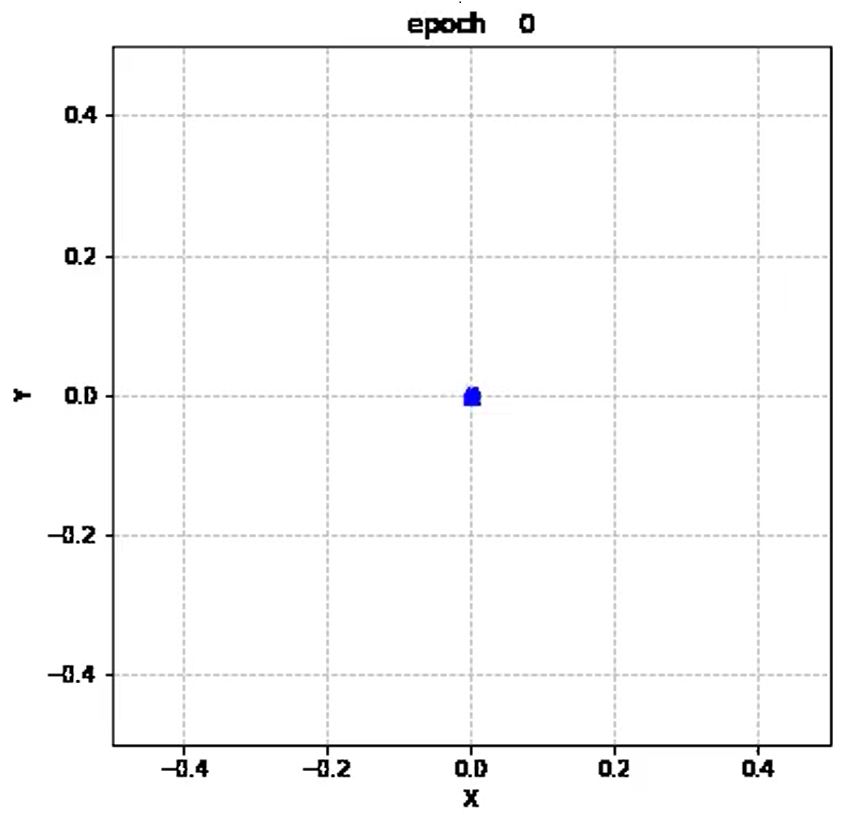
\includegraphics[width=\textwidth]{img/Results/Dataset_3/Camera/0 Epoch.png}
        \caption{Camera positions at the start of training (0 epochs)}
        \label{fig:Image1}
    \end{subfigure}
    \hfill
    \begin{subfigure}{.47\textwidth} % Adjust the width as needed
        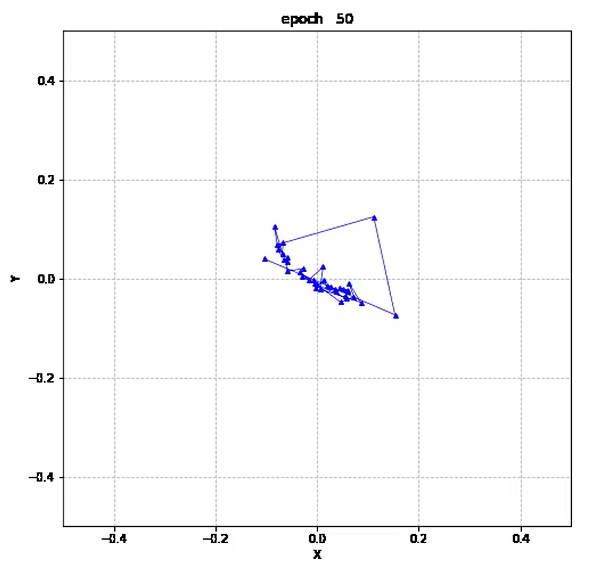
\includegraphics[width=\textwidth]{img/Results/Dataset_3/Camera/50 epochs.png}
        \caption{Camera positions after 50 epochs of training}
        \label{fig:Image2}
    \end{subfigure}
    \begin{subfigure}{.47\textwidth} % Adjust the width as needed
        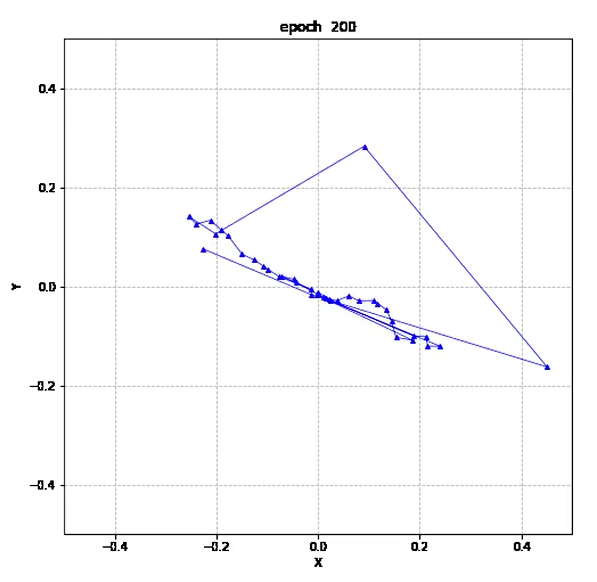
\includegraphics[width=\textwidth]{img/Results/Dataset_3/Camera/150 epochs.png}
        \caption{Camera positions after 200 epochs of training}
        \label{fig:Image3}
    \end{subfigure}
    \hfill
    \begin{subfigure}{.47\textwidth} % Adjust the width as needed
        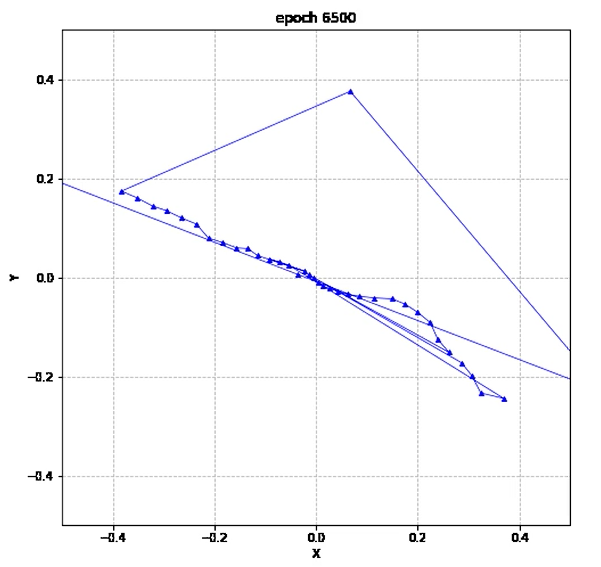
\includegraphics[width=\textwidth]{img/Results/Dataset_3/Camera/200 epochs.png}
        \caption{Camera positions after 6500 epochs of training}
        \label{fig:Image4}
    \end{subfigure}
    \caption{Progression of camera position optimization from 0 to 10,000 epochs in Dataset 3}
    \label{fig:Camera Position Optimization}
\end{figure}

\clearpage
\subsection{Dataset 3: Exploring Different Activation Functions}
Within our model, the primary activation function employed is the widely used \textbf{ReLU} (Rectified Linear Unit). However, we embarked on an exploration to investigate if there existed room for improvement in this crucial aspect. Our exploration involved the thorough examination of various alternative activation functions that have shown promise in image denoising tasks from NAN-NeRF \cite{Pearl2022}.

\vspace{10pt}
To efficiently conduct our experiments, we initially executed them for 200 epochs, considering that training for 10,000 epochs demanded an extensive time investment of over 10 hours. This initial phase served as a screening process, allowing us to identify any promising results within a shorter timeframe. Subsequently, if any of these early experiments yielded favorable outcomes in terms of PSNR or SSIM values, we proceeded with the full 10,000-epoch training to assess if further improvements could be achieved.

\subsubsection{1. Tahn activation function:}
\begin{figure}[H]
    \centering
    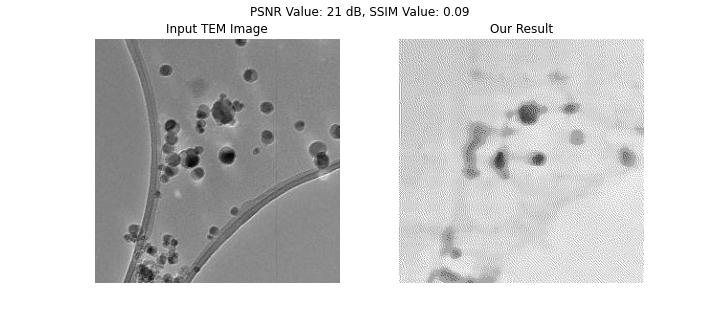
\includegraphics[width=1\textwidth]{img/Dataset_3_with_200_epochs_Activation_Function.jpg}
    \caption{Dataset 3 with Tanh Activation function (200 epochs).}\label{fig:Dataset_3_with_Tanh_200_epochs.jpg}
\end{figure}

We initiated our exploration of alternative activation functions by training the model using the \textbf{Tanh} activation function for a limited 200 epochs. In this initial phase, the results indicated a PSNR value of 21 dB and an SSIM value of 0.09. Recognizing the potential for improvement, we extended the training duration to 10,000 epochs, resulting in a significant enhancement in performance. The model achieved a remarkable PSNR value of 28.30 dB and an SSIM value of 0.16.

\vspace{10pt}

While the performance boost with \textbf{Tanh} activation was notable, it's worth noting that our original choice of \textbf{ReLU} still outperformed it, consistently delivering the highest PSNR value of 28.37 dB. This comparison underscored the efficacy of \textbf{ReLU} in our model's context.
\begin{figure}[H]
    \centering
    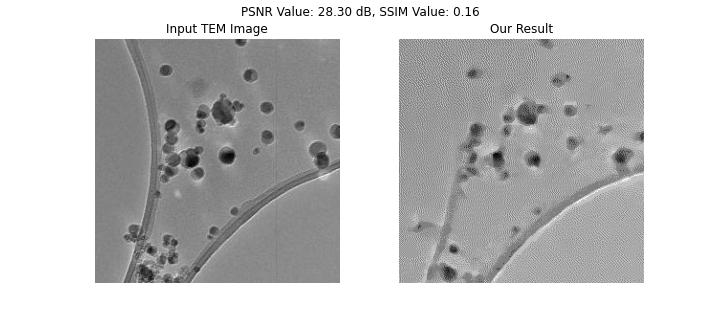
\includegraphics[width=1\textwidth]{img/Dataset_3_with_1000_epochs_Tanh_Activation_Function.jpg}
    \caption{Dataset 3 with Tanh Activation function (10,000 epochs).}\label{fig:Dataset_3_with_Tanh_10000_epochs.jpg}
\end{figure}

\subsubsection{2. Sigmoid activation function:}


In our experimental trials, we investigated the use of the \textbf{Sigmoid} activation function, initially training it for 200 epochs. However, this initial attempt yielded underwhelming results, as we did not calculate PSNR and SSIM values. Due to this lackluster performance in the early stages, we chose not to continue further experiments with the \textbf{Sigmoid} activation function and refrained from extending the training duration to 10,000 epochs.

\begin{figure}[H]
    \centering
    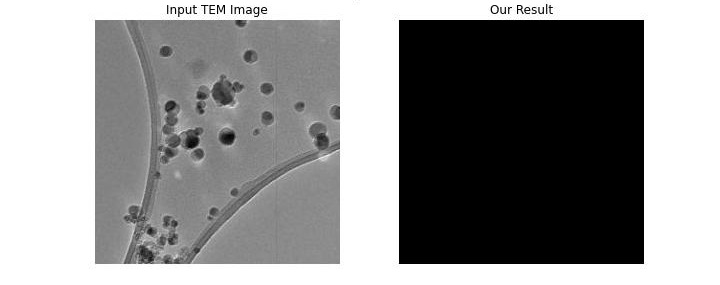
\includegraphics[width=1\textwidth]{img/Dataset_3_with_200_epochs_Sigmoid.jpg}
    \caption{Dataset 3 with Sigmoid Activation function (200 epochs).}\label{fig:Dataset_3_with_Sigmoid_200_epochs.jpg}
\end{figure}

\subsubsection{3. Leaky ReLU activation function:}
Our exploration into activation functions culminated with the \textbf{Leaky ReLU} activation function. We initiated this experiment with 200 epochs and were pleasantly surprised by the results, which yielded a remarkable 28.30 dB PSNR value and a 0.16 SSIM value. Encouraged by this promising outcome, we decided to further investigate the potential of \textbf{Leaky ReLU} by extending the training to 10,000 epochs, despite the substantial time investment required.

\begin{figure}[H]
    \centering
    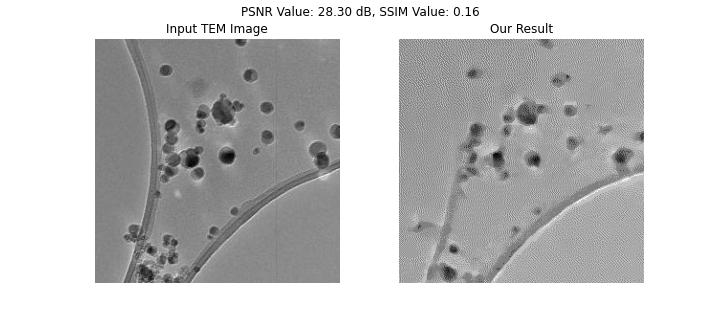
\includegraphics[width=1\textwidth]{img/Dataset_3_with_200_epochs_Leaky_Activation_Function.jpg}
    \caption{Dataset 3 with Leaky ReLU Activation function (200 epochs).}\label{fig:Dataset_3_with_Leaky_ReLU_200_epochs.jpg}
\end{figure}



\vspace{10pt}
The extended training period, spanning over 10 hours, proved to be worthwhile. The PSNR value exhibited significant improvement, increasing from 28.30 dB to 28.38 dB. Even more noteworthy was the enhancement in the SSIM value, which escalated to 0.18. This achievement surpassed the performance of the original \textbf{ReLU} activation function, prompting us to adopt \textbf{Leaky ReLU} as the final activation function for our model.

\begin{figure}[H]
    \centering
    \includegraphics[width=.9\textwidth]{img/Dataset_3_with_1000_epochs_Leaky_ReLU.jpg}
    \caption{Dataset 3 with  Leaky ReLU Activation function (10,000 epochs).}\label{fig:Dataset_3_with_Leaky_ReLU_10000_epochs.jpg}
\end{figure}

\subsection{Dataset 3 with different Network layer}
Our model initially consisted of a baseline configuration with a 4-layer neural network. In pursuit of improved performance, we conducted experiments to explore the impact of increasing the depth of our model. By incrementing the number of layers to 8, we witnessed a substantial enhancement in results \ref{fig:Dataset 3 0 to 10000 epochs PSNR values(Final)}.
\vspace{10pt}

The model with 8 layers achieved a noteworthy PSNR value of 29.84 dB and an SSIM value of 0.21. This outcome signified a significant improvement in the model's capacity to denoise and reconstruct images. The increased depth of the neural network contributed to the model's ability to capture more intricate patterns and details in the images, resulting in superior image quality.

\begin{figure}[H]
    \centering
    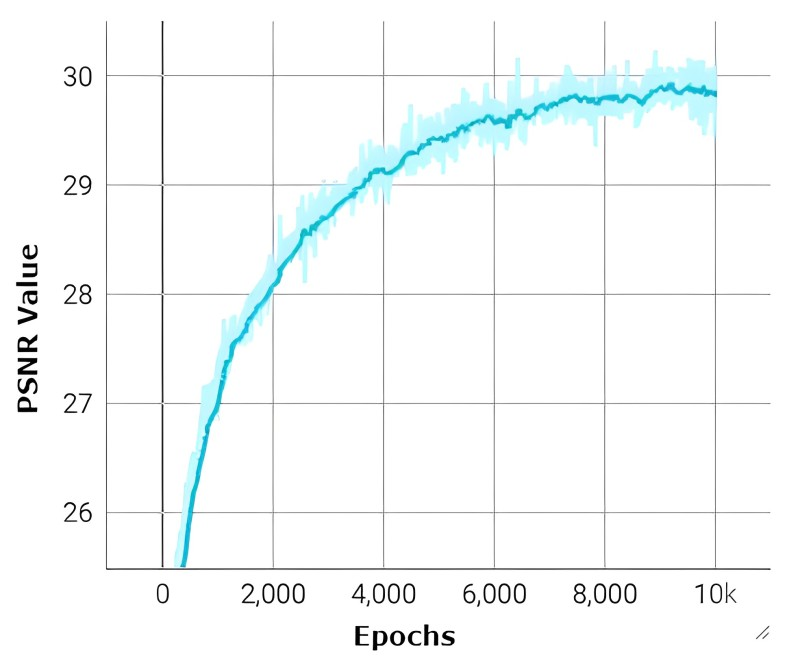
\includegraphics[width=.7\textwidth]{img/Final 10K PSNR graph.jpg}
    \caption{Progression of PSNR values over 10,000 epochs after adjusting hyperparameters for Dataset 3}\label{fig:Dataset 3 0 to 10000 epochs PSNR values(Final)}
\end{figure}

\begin{figure}[H]
    \centering
    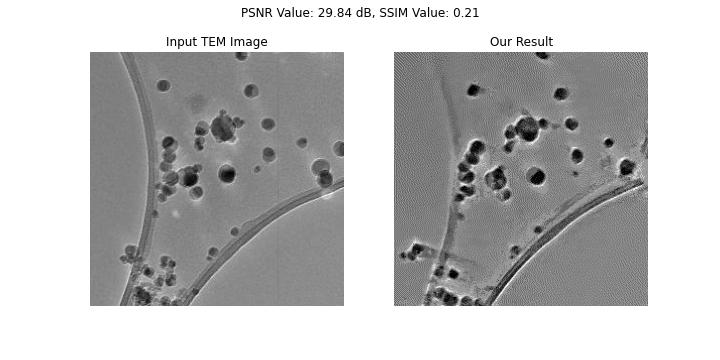
\includegraphics[width=.9\textwidth]{img/Dataset_3_with_8_Layer.jpg}
    \caption{Dataset 3 with  8 Layer Architecture.}\label{fig:Dataset_3_with_8_layer.jpg}
\end{figure}




\subsection{Enhancing the Model with NeRF-Dark and NAN-NeRF Parameters}

Incorporating advanced techniques from NeRF-Dark and NAN-NeRF, we enhanced the quality of our image reconstructions, as detailed in \ref{ch:Methodology} and \ref{ch:Implementation}. NeRF-Dark \cite{Mildenhall2021}, addressed the challenges of low-light conditions, common in TEM imaging. It enabled us to reconstruct high-quality images from previously unusable data. Additionally, NAN-NeRF \cite{Pearl2022}, excelled at nanoscale imaging, facilitating precise 3D reconstructions from limited and noisy TEM data. These innovations culminated in impressive results, with our images achieving a peak PSNR value of 31.29 dB and an SSIM value of 0.56, showcasing enhanced clarity and reduced noise.
\begin{figure}[H]
    \centering
    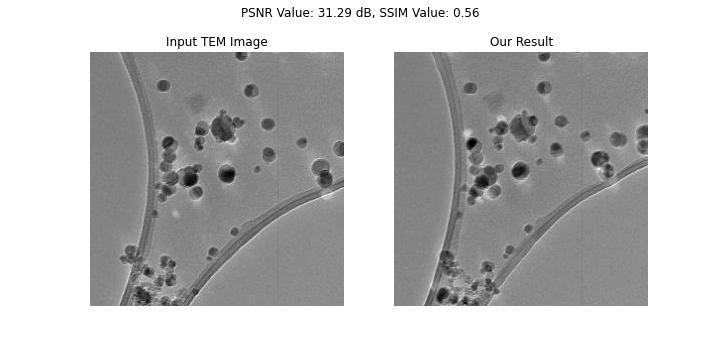
\includegraphics[width=.9\textwidth]{img/Dataset_3_with_Nerf_inthe_dark.jpg}
    \caption{Remarkable Enhancements in Image Quality Through NeRF-Dark and NAN-NeRF Integration.}\label{fig:Dataset_3_Nerf_inthe_dark.jpg}
\end{figure}

\subsection{Postprocessing with Traditional Denoisers}
In this section, we present the results of our experiments with traditional denoising techniques, as explained in Chapter \ref{ch:Methodology}. We evaluated methods including Bilateral Filtering, Gaussian Blur, Median Filtering, Non-Local Means Denoising, and Wavelet Denoising. Chosen for their established utility, these techniques range from Bilateral Filtering, known for edge preservation, to Wavelet Denoising, recognized for its selective denoising capability. The subsequent subsections detail the application of these methods to Dataset 3, showcasing the resulting postprocessed images and discussing their effectiveness.

\subsubsection{1. Bilateral Filtering}
Bilateral Filtering is a sophisticated denoising technique that excels in enhancing image quality by preserving edges and fine details while effectively reducing noise. In our experiment with Dataset 3, \textbf{Bilateral Filtering} achieved a PSNR value of \textbf{29.33 dB} and an SSIM value of \textbf{0.56}. These results highlight its capability to significantly improve image clarity and the discernibility of individual elements within the image.

\begin{figure}[H]
\centering
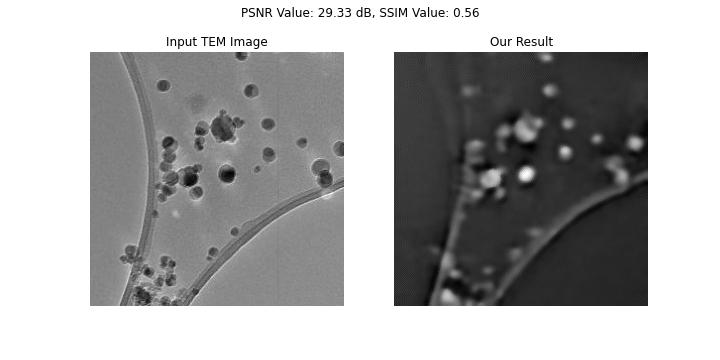
\includegraphics[width=1\textwidth]{img/Dataset_3_with_bilateral_filter.jpg}
\caption{Image Postprocessed with Bilateral Filtering.}\label{fig:Dataset_3_Bilateral_Filtering}
\end{figure}

\subsubsection{2. Gaussian Blur}
Gaussian Blur is a widely used denoising approach that aims to reduce noise by averaging pixel values within a specified radius. In our experiment, \textbf{Gaussian Blur} produced results similar to Bilateral Filtering, with a PSNR value of \textbf{29.33 dB} and an SSIM value of \textbf{0.56}. While the performance closely aligns with that of Bilateral Filtering, Gaussian Blur remains a viable option for noise reduction.

\begin{figure}[H]
\centering
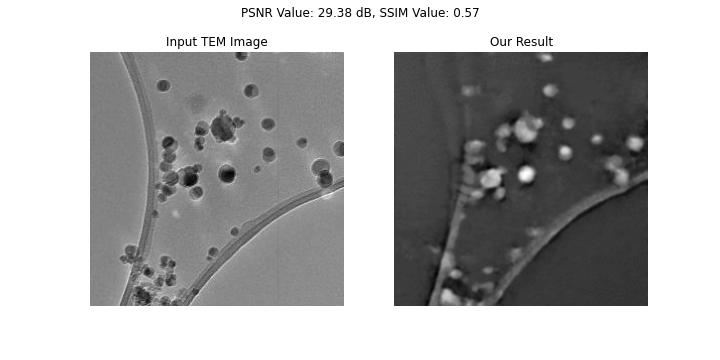
\includegraphics[width=1\textwidth]{img/Dataset_3_with_gaussian_blur.jpg}
\caption{Image Postprocessed with Gaussian Blur.}\label{fig:Dataset_3_Gaussian_Blur}
\end{figure}

\subsubsection{3. Median Filtering}
Median Filtering is a technique that effectively reduces noise while preserving image edges and structural details. It calculates the median value of neighboring pixels, making it robust against outliers. In our experiment, \textbf{Median Filtering} achieved a PSNR value of \textbf{29.03 dB} and an SSIM value of \textbf{0.52}. These results demonstrate its effectiveness in enhancing image quality by improving particle visibility and edge definition.

\begin{figure}[H]
\centering
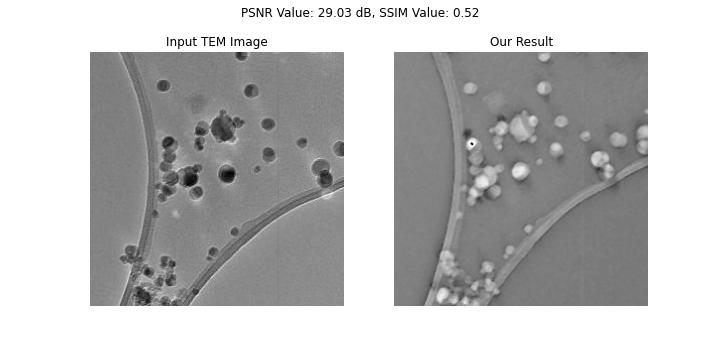
\includegraphics[width=.9\textwidth]{img/Dataset_3_with_median_filter.jpg}
\caption{Image Postprocessed with Median Filtering.}\label{fig:Dataset_3_Median_Filtering}
\end{figure}

\subsubsection{4. Non-Local Means Denoising}
Non-Local Means Denoising is a powerful technique known for its ability to effectively reduce noise while preserving image details. In our experiment, it achieved a remarkable PSNR value of \textbf{31.78 dB} and an SSIM value of \textbf{0.64}. However, the resulting image appeared slightly blurry, indicating a trade-off between noise reduction and image sharpness. Despite this trade-off, Non-Local Means Denoising remains a valuable tool for noise reduction tasks.

\begin{figure}[H]
\centering
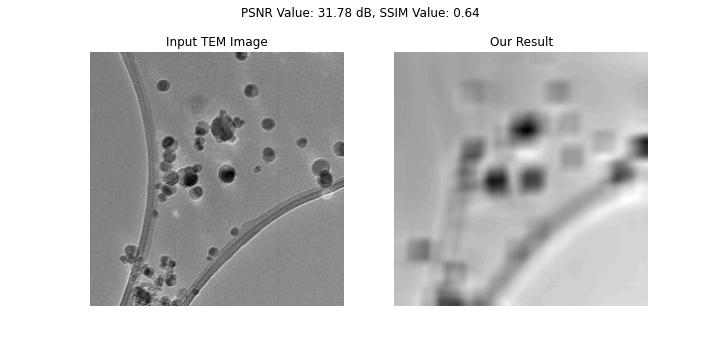
\includegraphics[width=.9\textwidth]{img/Dataset_3_with_non_local_means.jpg}
\caption{Image Postprocessed with Non-Local Means Denoising.}\label{fig:Dataset_3_Non_Local_Means_Denoising}
\end{figure}

\subsubsection{5. Wavelet Denoising}
Wavelet Denoising is a sophisticated denoising technique that excels in noise reduction while preserving image details. It decomposes the image into different frequency components and applies denoising selectively. In our experiment,\textbf{ Wavelet Denoising} outperformed the other techniques, achieving a PSNR value of\textbf{ 32.29 dB} and an impressive SSIM value of\textbf{ 0.68}. These results highlight its effectiveness in reducing noise and enhancing image quality, making it the preferred choice for Dataset 3.

\begin{figure}[H]
\centering
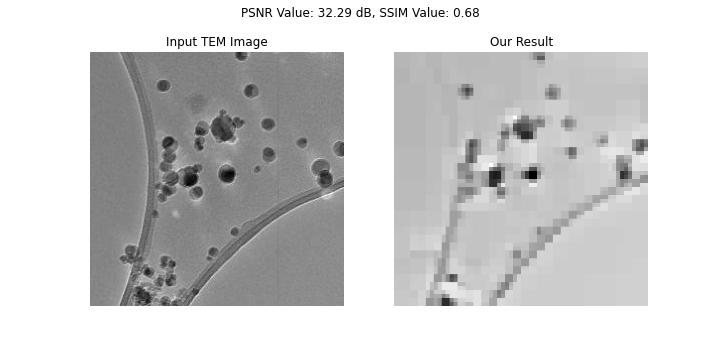
\includegraphics[width=.9\textwidth]{img/Dataset_3_with_wavelet.jpg}
\caption{Image Postprocessed with Wavelet Denoising.}\label{fig:Dataset_3_Wavelet_Denoising}
\end{figure}

Among the five denoising techniques evaluated for Dataset 3, Wavelet Denoising emerged as the top performer, achieving a PSNR value of 32.29 dB and an SSIM value of 0.68. This makes Wavelet Denoising the preferred choice for enhancing the image quality of Dataset 3.

\subsection{Postprocessing with ESRGAN}
The final stage of our image enhancement architecture involves the application of Enhanced Super-Resolution Generative Adversarial Networks (ESRGAN). ESRGAN is a powerful method that can infer high-resolution images up to four times larger than the input, making it superior to traditional denoising techniques. In this stage, we take the noisy and relatively small images generated by our model's output and significantly enhance their quality.

\begin{figure}[H]
\centering
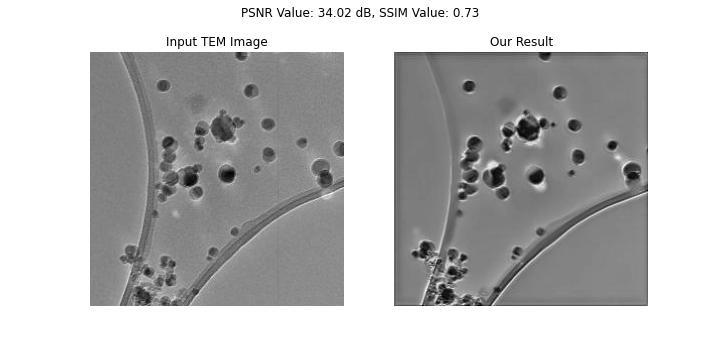
\includegraphics[width=.9\textwidth]{img/Dataset_3_with_ESRGAN.jpg}
\caption{Image Postprocessed with ESRGAN.}\label{fig:Dataset_3_ESRGAN}
\end{figure}

\vspace{10pt}

\textbf{ESRGAN} has proven to be highly effective, achieving exceptional results in terms of both objective image quality metrics and perceptual quality. Specifically, \textbf{ESRGAN} yielded a remarkable \textbf{PSNR} value of \textbf{34.02 dB} and an impressive \textbf{SSIM} value of\textbf{ 0.73}. These metrics represent the highest values obtained throughout our entire experimentation process.

\vspace{10pt}

From a visual perspective, the images postprocessed with ESRGAN exhibit several noteworthy characteristics. First and foremost, the images are notably sharp, with enhanced clarity and well-defined edges. This sharpness extends to even the smallest particles within the image, further emphasizing the effectiveness of noise reduction. Moreover, ESRGAN excels in eliminating noisy artifacts from the background, resulting in cleaner and more visually pleasing images.

\vspace{10pt}

This strategic utilization of ESRGAN as the final step in our image processing pipeline culminates in exceptional outcomes, ensuring that our reconstructed TEM images exhibit the highest levels of clarity, fidelity, and noise reduction.


\clearpage
\section{Experimental Analysis with TEM Dataset 1}
In our experiments with Dataset 1 \ref{fig:TEM Dataset 1}, we initially expected ESRGAN to outperform other methods. However, the Non-Local Means algorithm delivered surprisingly superior results in this dataset.

\vspace{10pt}

Non-Local Means \ref{fig:TEM_1_Image4} achieved a PSNR value of 33.02 dB and an SSIM value of 0.80, surpassing ESRGAN, which had a PSNR of 31.07 dB and SSIM of 0.38. This outcome can be attributed to the dataset's predominantly black background, which favored Non-Local Means and Wavelet denoising, with a PSNR of 33.00 dB and an SSIM of 0.79.

\vspace{10pt}

In contrast, the other three denoising algorithms did not yield notably remarkable results, making them less relevant in this context. Therefore, we focused our attention on the outstanding performance of Non-Local Means and Wavelet denoising for Dataset 1.


\begin{figure}[H]
    \centering
    \begin{subfigure}{.47\textwidth} % Adjust the width as needed
        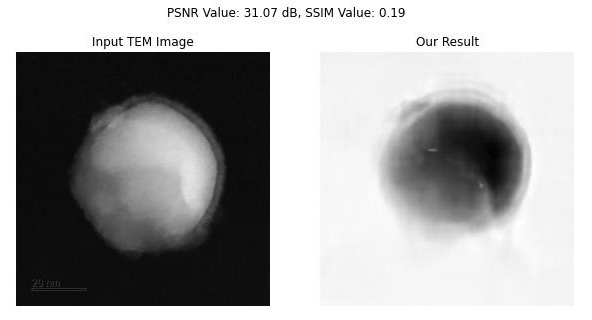
\includegraphics[width=\textwidth]{img/Results/Dataset_1/Dataset_1_Bila_filter.jpg}
        \caption{Applying Bilateral filter}
        \label{fig:Image1}
    \end{subfigure}
    \hfill
    \begin{subfigure}{.47\textwidth} % Adjust the width as needed
        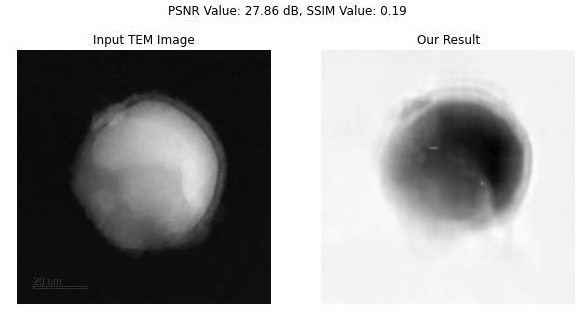
\includegraphics[width=\textwidth]{img/Results/Dataset_1/Dataset_1_gaussian_blur.jpg}
        \caption{Applying Gaussian Blur}
        \label{fig:Image2}
    \end{subfigure}
    
    \vspace{15pt} % Add vertical space between rows of subfigures
    
    \begin{subfigure}{.47\textwidth} % Adjust the width as needed
        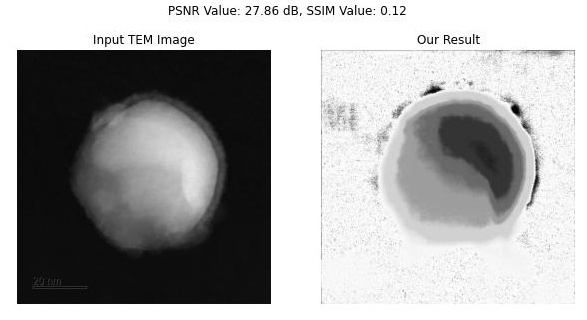
\includegraphics[width=\textwidth]{img/Results/Dataset_1/Dataset_1_median_filter.jpg}
        \caption{Applying Median Filter}
        \label{fig:Image3}
    \end{subfigure}
    \hfill
    \begin{subfigure}{.47\textwidth} % Adjust the width as needed
        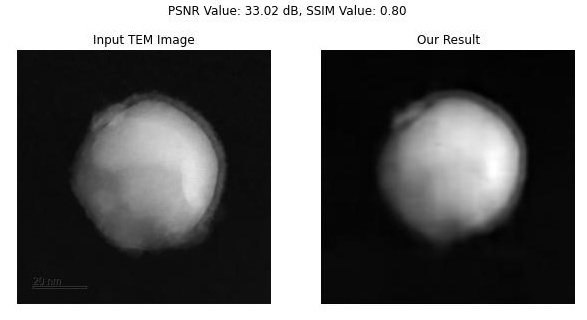
\includegraphics[width=\textwidth]{img/Results/Dataset_1/Dataset_1_non_local_means.jpg}
        \caption{Applying Non Local means}
        \label{fig:TEM_1_Image4}
    \end{subfigure}
    
    \vspace{15pt} % Add vertical space between rows of subfigures
    
    \begin{subfigure}{.47\textwidth} % Adjust the width as needed
        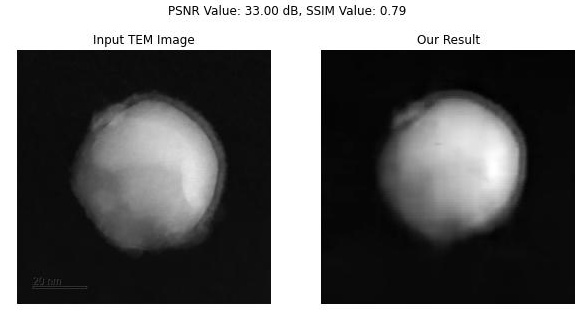
\includegraphics[width=\textwidth]{img/Results/Dataset_1/Dataset_1_wavelet.jpg}
        \caption{Applying Wavelet}
        \label{fig:Image5}
    \end{subfigure}
    \hfill
    \begin{subfigure}{.47\textwidth} % Adjust the width as needed
        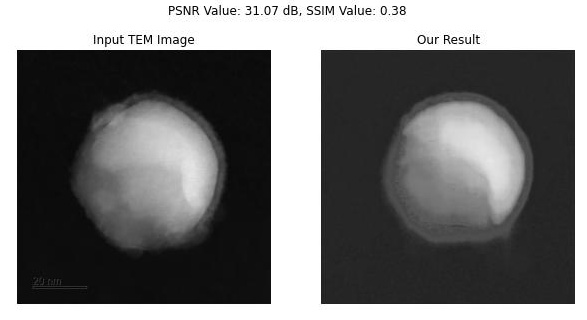
\includegraphics[width=\textwidth]{img/Results/Dataset_1/Dataset_1_ESRGAN.jpg}
        \caption{Applying ESRGAN}
        \label{fig:Image5}
    \end{subfigure}
    \caption{Experimental Results for TEM Dataset 1.}
    \label{fig:TEM_Dataset_1_Results}
\end{figure}


\clearpage
\section{Experimental Analysis with TEM Dataset 2}
TEM Dataset 2 (refer to Figure \ref{fig:TEM Dataset 2}) exhibited exceptional denoising capabilities, particularly in dark backgrounds. ESRGAN delivered astounding results with a PSNR value of 38.70 dB and an SSIM value of 0.95, nearing the highest possible SSIM value of 1. Furthermore, Non-Local Means and Wavelet denoising also showcased commendable performance, achieving PSNR values of 34.54 dB and 34.57 dB, with SSIM values of 0.75 and 0.74, respectively.
\vspace{10pt}

In contrast, Bilateral Filter, Gaussian Blur, and Median Filter yielded average results, with PSNR values around 29.00 dB and SSIM values of approximately 0.70.

\vspace{10pt}

The superiority of ESRGAN(refer to figure \ref{fig:TEM_Dataset_2_Image5}) in this dataset is evident, reaffirming its effectiveness in challenging denoising scenarios.



\begin{figure}[H]
    \centering
    \begin{subfigure}{.47\textwidth} % Adjust the width as needed
        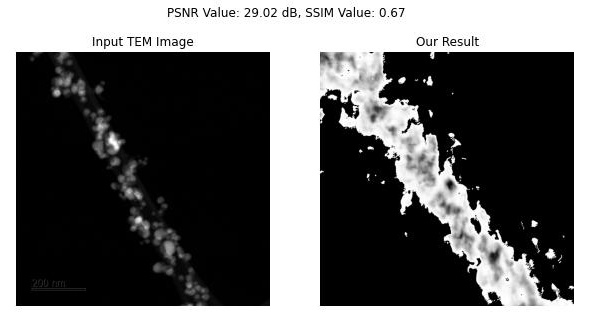
\includegraphics[width=\textwidth]{img/Results/Dataset_2/Dataset_2_bilateral_filter.jpg}
        \caption{Applying Bilateral filter}
        \label{fig:Image1}
    \end{subfigure}
    \hfill
    \begin{subfigure}{.47\textwidth} % Adjust the width as needed
        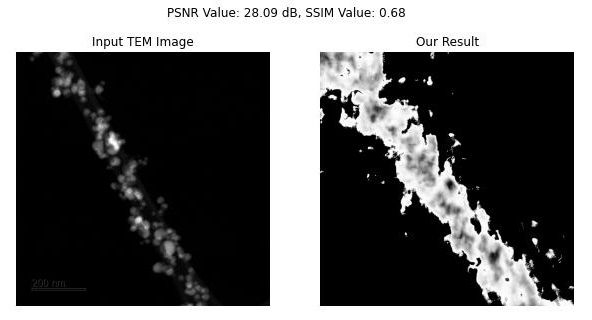
\includegraphics[width=\textwidth]{img/Results/Dataset_2/Dataset_2_gaussian_blur.jpg}
        \caption{Applying Gaussian Blur}
        \label{fig:Image2}
    \end{subfigure}
    
    \vspace{15pt} % Add vertical space between rows of subfigures
    
    \begin{subfigure}{.47\textwidth} % Adjust the width as needed
        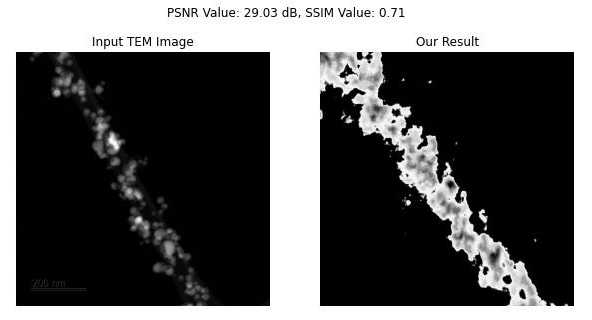
\includegraphics[width=\textwidth]{img/Results/Dataset_2/Dataset_2_median_filter.jpg}
        \caption{Applying Median Filter}
        \label{fig:Image3}
    \end{subfigure}
    \hfill
    \begin{subfigure}{.47\textwidth} % Adjust the width as needed
        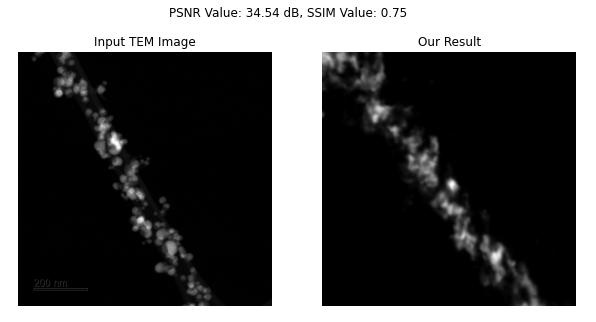
\includegraphics[width=\textwidth]{img/Results/Dataset_2/Dataset_2_non_local_means.jpg}
        \caption{Applying Non Local means}
        \label{fig:Image4}
    \end{subfigure}
    
    \vspace{15pt} % Add vertical space between rows of subfigures
    
    \begin{subfigure}{.47\textwidth} % Adjust the width as needed
        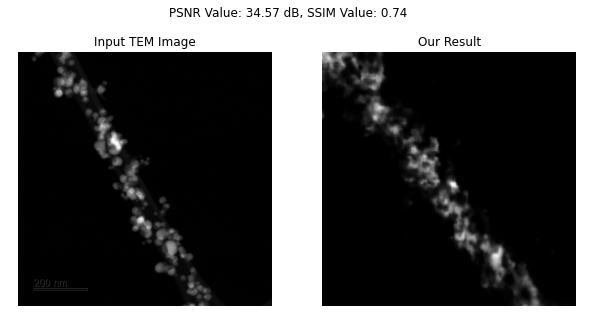
\includegraphics[width=\textwidth]{img/Results/Dataset_2/Dataset_2_wavelet.jpg}
        \caption{Applying Wavelet}
        \label{fig:Image5}
    \end{subfigure}
    \hfill
    \begin{subfigure}{.47\textwidth} % Adjust the width as needed
        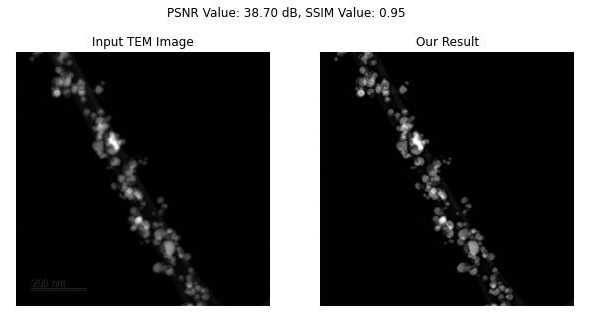
\includegraphics[width=\textwidth]{img/Results/Dataset_2/Dataset_2_ESRGAN.jpg}
        \caption{Applying ESRGAN}
        \label{fig:TEM_Dataset_2_Image5}
    \end{subfigure}
    \caption{Experimental Results for TEM Dataset 2}
    \label{fig:TEM_Dataset_2_Results}
\end{figure}


\clearpage
\section{Experimental Analysis with TEM Dataset 4}
TEM Dataset 4, shown in Figure \ref{fig:TEM Dataset 4}, consists of sharply structured particles against a gray background, aiding our model in 3D structure reconstruction. Its larger size of 1421 x 1421 pixels poses unique image processing challenges.
\vspace{10pt}

Regarding denoising performance, ESRGAN \ref{fig:TEM_Dataset_4_Image5} excelled with the highest PSNR value of 31.56dB and an SSIM of 0.72, indicating superior image quality enhancement. The Wavelet method also performed comparably, achieving a PSNR of 31.50dB and an SSIM of 0.70, demonstrating its effectiveness in noise reduction.
\vspace{10pt}

The Non-Local method yielded a PSNR of 31.45dB and an SSIM of 0.70, closely matching the Wavelet's results and proving its efficiency. Meanwhile, the other three algorithms averaged a PSNR of around 29.50dB and an SSIM of 0.60, reflecting good image quality improvement, albeit slightly lower than the leading methods.


\begin{figure}[H]
    \centering
    \begin{subfigure}{.47\textwidth} % Adjust the width as needed
        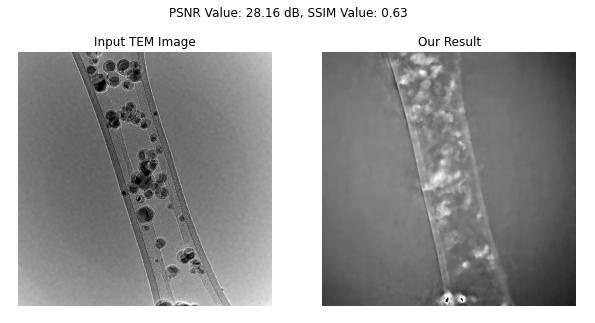
\includegraphics[width=\textwidth]{img/Results/Dataset_4/Dataset_4_bilateral_filter.jpg}
        \caption{Applying Bilateral filter}
        \label{fig:Image1}
    \end{subfigure}
    \hfill
    \begin{subfigure}{.47\textwidth} % Adjust the width as needed
        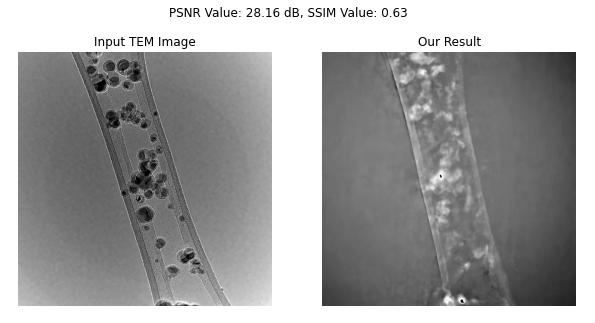
\includegraphics[width=\textwidth]{img/Results/Dataset_4/Dataset_4_gaussian_blur.jpg}
        \caption{Applying Gaussian Blur}
        \label{fig:Image2}
    \end{subfigure}
    
    \vspace{15pt} % Add vertical space between rows of subfigures
    
    \begin{subfigure}{.47\textwidth} % Adjust the width as needed
        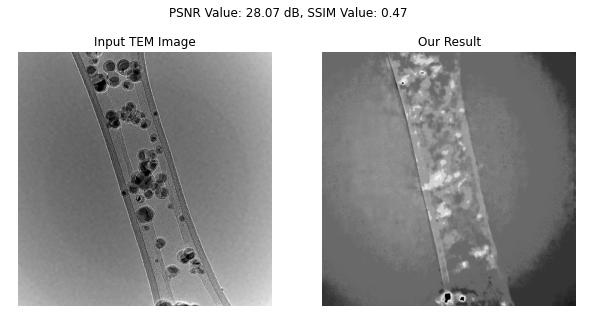
\includegraphics[width=\textwidth]{img/Results/Dataset_4/Dataset_4_median_filter.jpg}
        \caption{Applying Median Filter}
        \label{fig:Image3}
    \end{subfigure}
    \hfill
    \begin{subfigure}{.47\textwidth} % Adjust the width as needed
        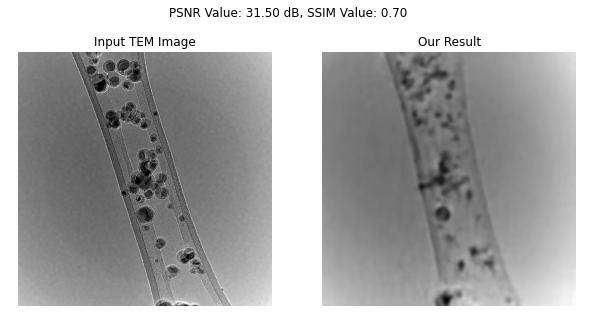
\includegraphics[width=\textwidth]{img/Results/Dataset_4/Dataset_4_non_local_means.jpg}
        \caption{Applying Non Local means}
        \label{fig:Image4}
    \end{subfigure}
    
    \vspace{15pt} % Add vertical space between rows of subfigures
    
    \begin{subfigure}{.47\textwidth} % Adjust the width as needed
        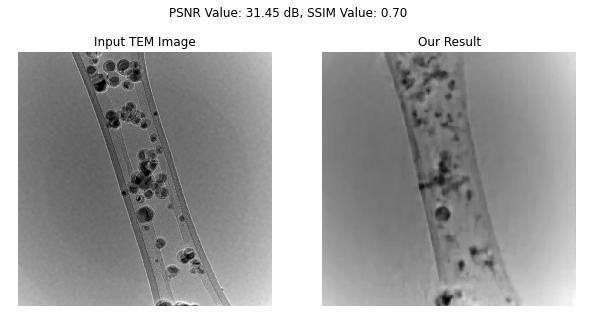
\includegraphics[width=\textwidth]{img/Results/Dataset_4/Dataset_4_wavelet.jpg}
        \caption{Applying Wavelet}
        \label{fig:Image5}
    \end{subfigure}
    \hfill
    \begin{subfigure}{.47\textwidth} % Adjust the width as needed
        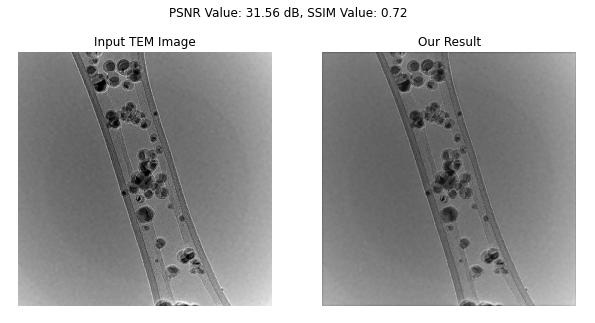
\includegraphics[width=\textwidth]{img/Results/Dataset_4/Dataset_4_ESRGAN.jpg}
        \caption{Applying ESRGAN}
        \label{fig:TEM_Dataset_4_Image5}
    \end{subfigure}
    \caption{Experimental Results for TEM Dataset 4}
    \label{fig:TEM_Dataset_4_Results}
\end{figure}


\clearpage
\section{Experimental Analysis with STEM Dataset 1}
Figure \ref{fig:STEM Dataset 1} shows STEM Dataset 1, featuring a single particle with solid material attachment, posing a unique challenge in image processing. This dataset is the largest we tested, with images of 1024 x 1024 pixels, each about 1 MB.

\vspace{10pt}
Unexpectedly, ESRGAN registered the lowest PSNR at 25.06 dB in our experiments, while Wavelet \ref{fig:STEM_Dataset_1_Results_Image5} and Non-Local means \ref{fig:STEM_Dataset_1_Results_Image4} excelled with PSNRs of 34.45 and 34.42, respectively. In terms of SSIM, Non-Local means led with 0.84, followed by Wavelet at 0.83, indicating strong structural preservation. Despite its low PSNR, ESRGAN achieved a better SSIM of 0.62, suggesting decent structure retention. The Gaussian blur had the lowest SSIM at 0.10, and Bilateral Filter and Median methods showed moderate PSNR but lower SSIM values, close to the Gaussian blur's performance.



\begin{figure}[H]
    \centering
    \begin{subfigure}{.47\textwidth} % Adjust the width as needed
        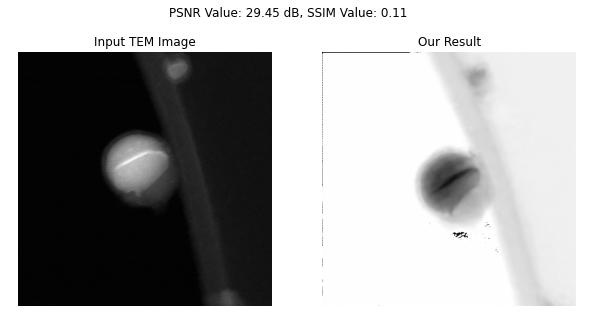
\includegraphics[width=\textwidth]{img/Results/STEM dataset 1/STEM_Data_1_bilateral_filter.jpg}
        \caption{Applying Bilateral filter}
        \label{fig:Image1}
    \end{subfigure}
    \hfill
    \begin{subfigure}{.47\textwidth} % Adjust the width as needed
        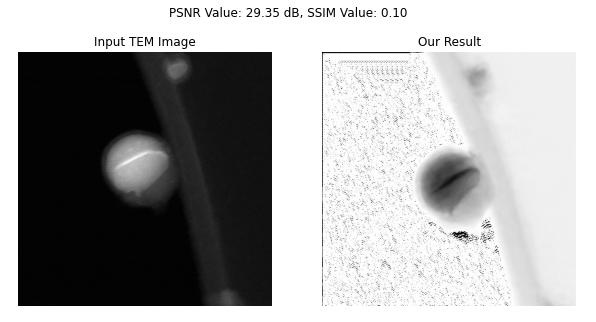
\includegraphics[width=\textwidth]{img/Results/STEM dataset 1/STEM_Data_1_gaussian_blur.jpg}
        \caption{Applying Gaussian Blur}
        \label{fig:Image2}
    \end{subfigure}
    
    \vspace{15pt} % Add vertical space between rows of subfigures
    
    \begin{subfigure}{.47\textwidth} % Adjust the width as needed
        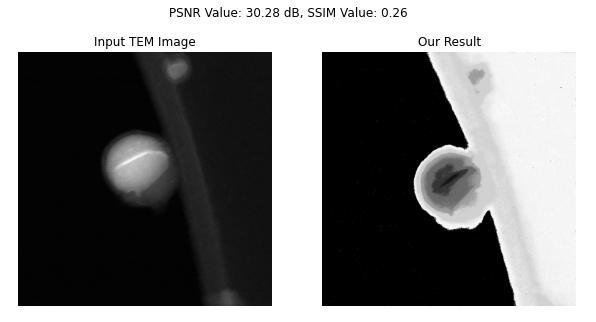
\includegraphics[width=\textwidth]{img/Results/STEM dataset 1/STEM_Data_1_median_filter.jpg}
        \caption{Applying Median Filter}
        \label{fig:Image3}
    \end{subfigure}
    \hfill
    \begin{subfigure}{.47\textwidth} % Adjust the width as needed
        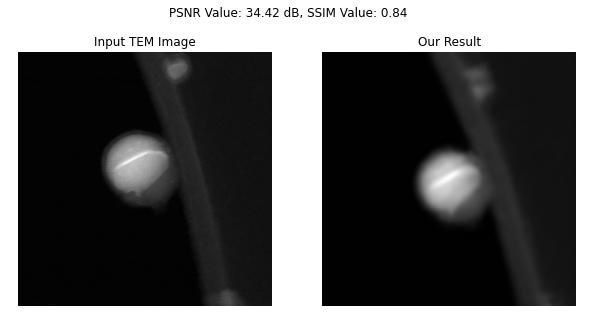
\includegraphics[width=\textwidth]{img/Results/STEM dataset 1/STEM_Data_1_non_local_means.jpg}
        \caption{Applying Non Local means}
        \label{fig:STEM_Dataset_1_Results_Image4}
    \end{subfigure}
    
    \vspace{15pt} % Add vertical space between rows of subfigures
    
    \begin{subfigure}{.47\textwidth} % Adjust the width as needed
        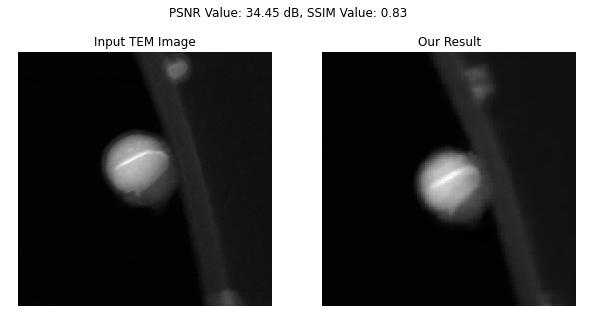
\includegraphics[width=\textwidth]{img/Results/STEM dataset 1/STEM_Data_1_wavelet.jpg}
        \caption{Applying Wavelet}
        \label{fig:STEM_Dataset_1_Results_Image5}
    \end{subfigure}
    \hfill
    \begin{subfigure}{.47\textwidth} % Adjust the width as needed
        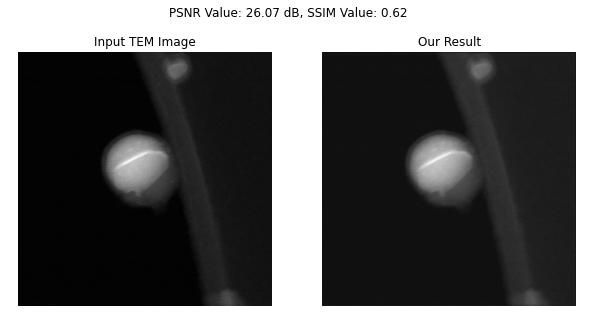
\includegraphics[width=\textwidth]{img/Results/STEM dataset 1/STEM_Data_1_ESRGAN.jpg}
        \caption{Applying ESRGAN}
        \label{fig:Image5}
    \end{subfigure}
    \caption{Experimental Results for STEM Dataset 1}
    \label{fig:STEM_Dataset_1_Results}
\end{figure}

\clearpage
\section{Experimental Analysis with STEM Dataset 2}
STEM Dataset 2 \ref{fig:STEM Dataset 2} represents a challenging experiment that yielded unsatisfactory results. Our Method architecture, which is designed to generate 3D reconstructions from input images, produced completely dark outputs for this dataset. Upon closer examination of STEM Dataset 2 \ref{fig:STEM Dataset 2}, it becomes apparent that the dataset features a predominantly black and dark background. The images exhibit high levels of noise and generally poor image quality. Notably, all images in this dataset have a file size of 60KB and a resolution of 1024 x 1024 pixels, where our model effectively renders every pixel as a dark point.

\vspace{10pt}
A closer inspection of the initial camera position optimization in \ref{fig:STEM2Image1} reveals that the camera remains fixed at the (0,0) position. Even after 184 epochs, as shown in \ref{fig:STEM2Image2}, the camera position remains unchanged. This persistent stagnation indicates that our model struggles to detect any meaningful features within the images, resulting in a consistent camera position of (0,0) for all images. Consequently, this dataset experiment can be deemed a failure due to the inability of our model to discern relevant information within the images.

\begin{figure}[H]
\centering
    \begin{subfigure}{.47\textwidth} % Adjust the width as needed
        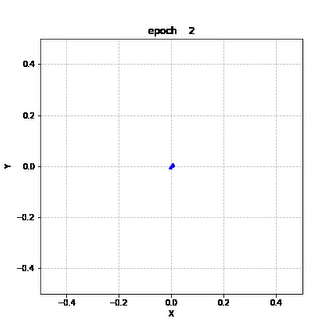
\includegraphics[width=\textwidth]{img/Results/STEM dataset 2/Screenshot 2023-12-23 164741.png}
        \caption{Visualization of Camera Position Optimization After 2 Epochs}
        \label{fig:STEM2Image1}
    \end{subfigure}
    \hfill
    \begin{subfigure}{.47\textwidth} % Adjust the width as needed
        \includegraphics[width=\textwidth]{img/Results/STEM dataset 2/Screenshot 2023-12-23 164924.png}
        \caption{Visualization of Camera Position Optimization After 184 Epochs}
        \label{fig:STEM2Image2}
    \end{subfigure}
    \caption{Experimental Results for STEM Dataset 2}
    \label{fig:STEM_Dataset_1_Results}
\end{figure}


\clearpage
\section{Experimental Analysis with Synthetic Dataset}
Our Synthetic Dataset experiment aimed to test our model's ability to reconstruct 3D structures. Despite the data being cleaner and clearer, the image size was notably small, around 80KB. This contrasts with a similar small-sized dataset (see Figure \ref{fig:STEM Dataset 2}), where our model struggled to generate 3D structures. However, with 120 images in the Synthetic Dataset, we observed a positive outcome, as demonstrated in Figure \ref{fig:Still Frames from Video Generated Using 2D Images with New Camera Angle}, showing that our model can leverage a larger number of smaller images.

\vspace{10pt}
We successfully generated a 3D structure from the Synthetic Dataset, and our methods yielded impressive results. ESRGAN achieved the highest PSNR of 34.56 (see Figure \ref{fig:Synthetic_Dataset_Results_Image5}) with an SSIM of 0.75. Wavelet (Figure \ref{fig:Synthetic_Dataset_Results_Image5}) and Non-Local (Figure \ref{fig:Synthetic_Dataset_Results_Image4}) methods surpassed ESRGAN with SSIM values of 0.81 and 0.78, respectively. In contrast, Gaussian blur had the lowest PSNR at 26.19 dB, while Median means recorded the lowest SSIM at 0.41. 

\vspace{20pt}

\begin{figure}[H]
    \centering
    \begin{subfigure}{.47\textwidth} % Adjust the width as needed
        \includegraphics[width=\textwidth]{img/Results/Synthetic data/Blender_Data_4_bilateral_filter.jpg}
        \caption{Applying Bilateral filter}
        \label{fig:Image1}
    \end{subfigure}
    \hfill
    \begin{subfigure}{.47\textwidth} % Adjust the width as needed
        \includegraphics[width=\textwidth]{img/Results/Synthetic data/Blender_Data_4_gaussian_blur.jpg}
        \caption{Applying Gaussian Blur}
        \label{fig:Image2}
    \end{subfigure}
    
    \vspace{15pt} % Add vertical space between rows of subfigures
    
    \begin{subfigure}{.47\textwidth} % Adjust the width as needed
        \includegraphics[width=\textwidth]{img/Results/Synthetic data/Blender_Data_4_median_filter.jpg}
        \caption{Applying Median Filter}
        \label{fig:Image3}
    \end{subfigure}
    \hfill
    \begin{subfigure}{.47\textwidth} % Adjust the width as needed
        \includegraphics[width=\textwidth]{img/Results/Synthetic data/Blender_Data_4_non_local_means.jpg}
        \caption{Applying Non Local means}
        \label{fig:Synthetic_Dataset_Results_Image4}
    \end{subfigure}
    
    \vspace{15pt} % Add vertical space between rows of subfigures
    
    \begin{subfigure}{.47\textwidth} % Adjust the width as needed
        \includegraphics[width=\textwidth]{img/Results/Synthetic data/Blender_Data_4_wavelet.jpg}
        \caption{Applying Wavelet}
        \label{fig:Synthetic_Dataset_Results_Image5}
    \end{subfigure}
    \hfill
    \begin{subfigure}{.47\textwidth} % Adjust the width as needed
        \includegraphics[width=\textwidth]{img/Results/Synthetic data/Blender_Data_4_ESRGAN.jpg}
        \caption{Applying ESRGAN}
        \label{fig:Synthetic_Dataset_Results_Image5}
    \end{subfigure}
    \caption{Experimental Results for Synthetic Dataset}
    \label{fig:Synthetic_Dataset_Results}
\end{figure}

\clearpage
\section{Comparative PSNR \& SSIM Analysis of Image Denoising}

This overview presents the experimental results across all 8 datasets using our model. In the table, cells highlighted in \textbf{Green} indicate the \textbf{highest PSNR} and \textbf{highest SSIM} values for each dataset, while those in \textbf{Red} denote the \textbf{lowest} values.

\begin{table}[ht]
\centering
\renewcommand{\arraystretch}{1.5} % Adjust the height of each row
\small % Makes the font smaller; you can also use \footnotesize or \scriptsize
\begin{tabular}{|l|c|c|c|c|c|c|}
\hline
Datasets & Bilateral & Gaussian  & Median  & Non-Local & Wavelet & ESRGAN \\
\hline
TEM Dataset 1 & 31.07 & \lowest{27.86} &  27.84 &  \highest{33.02} & 33.00 & 31.07 \\
\hline
TEM Dataset 2 & 29.02 & \lowest{28.09} & 29.03 & 34.54 & 34.57 & \highest{38.70} \\
\hline
TEM Dataset 3 & 29.33 & 29.38 & \lowest{29.03} & 31.78 & 32.29 & \highest{34.02} \\
\hline
TEM Dataset 4 & 28.16 & 28.16 & \lowest{28.07} & 31.50 & 31.45 & \highest{31.56}\\
\hline
STEM Dataset 1 & 29.45 & 29.35 & 30.28 & 34.42 & \highest{34.45} & \lowest{26.07} \\
\hline
STEM Dataset 2 & X  & X  &  X & X  & X  & X \\
\hline
Synthetic Dataset & 28.02 & \lowest{26.19} & 30.35  & 33.4 & 33.05 & \highest{34.56} \\
\hline
\end{tabular}
\caption{Comparative Analysis of Image Denoising Techniques Across TEM and STEM Datasets Measured by \textbf{Peak Signal-to-Noise Ratio (PSNR)}}
\label{tab:denoising_results_PSNR}
\end{table}

\begin{table}[ht]
\centering
\renewcommand{\arraystretch}{1.5} % Adjust the height of each row
\small % Makes the font smaller; you can also use \footnotesize or \scriptsize
\begin{tabular}{|l|c|c|c|c|c|c|}
\hline
Datasets & Bilateral & Gaussian  & Median  & Non-Local & Wavelet & ESRGAN \\
\hline
TEM Dataset 1 & 0.19 & 0.19 &  \lowest{0.12} &  \highest{0.80} & 0.79 & 0.38 \\
\hline
TEM Dataset 2 & \lowest{0.67} & 0.68 & 0.71 & 0.75 & 0.74 & \highest{0.95} \\
\hline
TEM Dataset 3 & 0.56 & 0.57 & \lowest{0.52} & 0.64 & 0.68 & \highest{0.73} \\
\hline
TEM Dataset 4 & 0.63 & 0.63 & \lowest{0.47} & 0.70 & 0.70 & \highest{0.72}\\
\hline
STEM Dataset 1 & 0.11 & \lowest{0.10} & 0.26 & \highest{0.84} & 0.83 & 0.62 \\
\hline
STEM Dataset 2 & X  & X  &  X & X  & X  & X \\
\hline
Synthetic Dataset & 0.59 & 0.66 & \lowest{0.41}  & 0.78 & \highest{0.81} & 0.75 \\
\hline
\end{tabular}
\caption{Evaluation of Image Denoising Efficacy on Various Datasets Using the \textbf{Structural Similarity Index Measure (SSIM)}}

\label{tab:denoising_results_SSIM}
\end{table}



